\section{Final Desicion Logic}\label{sec:fdl:ufdl}

This description is for version \versionfdl of Final Desicion Logic.\\

The Final Desicion Logic (\ufdl) firmware contains algo-bx-masks, suppression of algos caused by calibration trigger, prescalers, veto-masks and rate-counters
("before prescalers", "after prescalers" and "post dead time") for each Algorithm and the local \finor- and veto-logic.

\begin{figure}[htb]
\centering
\includegraphics[width=15cm]{figures/mFDL_firmware}
\caption{\ufdl firmware}
\label{fig:fdl:mFDL_firmware}
\end{figure}

\subsection{\ufdl Interface}
\label{sec:fdl:ufdl_interface}

%\textit{under construction ...}

\textbf{Inputs:}
\begin{itemize}
\item Algorithms from \ugtl
\item IPBus interface (for registers, counters and memories)
\item LHC clock
\item Reset signal
\item BC0, BGo test-enable, L1A
% \item Indication of LHC gap
\item Begin of lumi-section
% \item Bx-nr for algo-bx-masks memory
\end{itemize}
\textbf{Outputs:}
\begin{itemize}
% \item Status information of \ufdl
\item Prescale factor set index to \rop
\item Algorithms after GTLogic to \rop
\item Algorithms after algo-bx-masks to \rop
\item Algorithms after prescalers to \rop
\item Algorithms after \finor-masks to \rop
\item Local \finor to \rop
\item Local veto to \rop
\item Local \finor with veto to \rop
\item Local \finor to mezzanine
\item Local veto to mezzanine
\item Local \finor with veto to mezzanine
\end{itemize}

\subsection{MP7 \finor hardware solution}

%% Text, figures and tables moved to com-hardware.tex
The firmware of \ufdl in this document is based on a hardware configuration with maximum 6 \ugt modules.
% A proposed hardware solution for \finor is documented in \ref{sec:com-hard:hw_config_finor_mp7}.

\subsection{Data flow}
\label{sec:fdl:data_flow}

\begin{figure}[htb]
\centering
\includegraphics[width=15cm]{figures/fdl_pipeline_v1_0_1}
\caption{\ufdl pipeline}
\label{fig:fdl:mFDL_pipeline}
\end{figure}

Every Algorithm, in total 512 coming from \ugtl, passes a algo-bx-mask, the logic for suppression of algos caused by calibration trigger (\ref{calibration_trigger_gap_reg}) and a prescaler, which reduces the trigger rate by a given factor. The factor has a precision of two digits after comma ("fractional prescale factor"). Prescaled Algorithms signals are combined to a local final-or-signal (\finor).
For every Algorithm there is a rate-counter before prescaler and after prescaler, which are incremented by LHC clock if the Algorithm is true. In addition there are post-dead-time counters, one for each Algorithm, which are incremented,
if the Algorithm and the L1A-signal are true at the same bunch-crossing.
Algorithms after GTLogic, after algo-bx-masks, after prescalers, the local \finor- and local Veto-signal are provided for read-out-record.\\
If there are not enough firmware resources in one \ugt board, more boards could be used. Therefore the 512 Algorithms are partitioned by TME. TME will set the number of Algorithms as
constant in the package module \texttt{gtl\_pkg.vhd}. This means \ugtl and \ufdl firmware considered as a unit for synthesis. In the case of more \ugt boards, the local \finor and local veto are routed via
a mezzanine board on MP7 (located on "General Purpose I/O connector") to the FINOR-AMC502 module, where the total \finor is created and send to TCDS.\\
A mapping for Algorithms is provided, to give flexibility for setting the index of Algorithms:
\begin {itemize}
\item creating a mapping instance (algo\_mapping\_rop.vhd) by VHDL Producer, this component will be instantiated in fix part of FDL, and new calculation will done each time over TME.
\item TME delivers just the number of Algorithms, which will be built on each card.
\item from FDL point of view, FDL see incremented number of Algorithms indexes, \eg 0, 1, 2, which is \eg 69, 200, 300.
\item TME should take care of assignment of each Algorithm to a number, that means if in card 1 algo\_59 is defined, nobody allows to produce the same number again.
\end {itemize}
% A software which manages these partitioned Algorithms for setting prescale factors, reading rate-counters and other accesses has to be developed.\\

\clearpage

\subsection{Implementation in firmware}
\label{sec:fdl:implementation_firmware}

The entity-declaration of \href{\gitbranch/firmware/hdl/payload/fdl_module.vhd}{\texttt{fdl\_module.vhd}} is shown in \ref{sec:fdl:data_flow}.\\

Listing~\ref{lst:fdl:fdl_module_vhd} contains the entity-declaration of the \texttt{fdl\_module.vhd}.\\

\lstinputlisting[label=lst:fdl:fdl_module_vhd,language=VHDL,caption=Entity declaration of \texttt{fdl\_module.vhd}]{interfaces/fdl_module.vhd}

\medskip
\begin{table}
\footnotesize
\caption{Explanation of Listing~\ref{lst:fdl:fdl_module_vhd}}
\vspace{5mm}
\centering
\begin{tabular}{l p{.7\columnwidth}}
\toprule
{Item} & {Explanation}\\
\midrule
\verb|SIM_MODE| & switch for simulation mode.\\
\verb|PRESCALE_FACTOR_INIT| & init value for prescale factor.\\
\verb|MASKS_INIT| & init value for BX mask.\\
\verb|PRESCALE_FACTOR_SET_INDEX_WIDTH| & width of prescale factor set index.\\
\verb|PRESCALE_FACTOR_SET_INDEX_REG_INIT| & init value prescale factor set index register.\\
\verb|L1A_LATENCY_DELAY_INIT| & init value of L1A latency delay.\\
\verb|CNTRL_REG_INIT| & init value control register.\\
\verb|ALGO_INPUTS_FF| & switch for algos input flip-flops.\\
\verb|ipb_clk| & IPBus clock input.\\
\verb|ipb_rst| & IPBus reset input.\\
\verb|ipb_in| & IPBus data input.\\
\verb|ipb_out| & IPBus data output.\\
\verb|lhc_clk| & clock input (LHC clock).\\
\verb|lhc_rst| & reset input.\\
\verb|bcres| & TTC BGo bunch counter reset input.\\
\verb|test_en| & TTC BGo test enable input.\\
\verb|l1a| & L1A input.\\
\verb|begin_lumi_section| & begin of lumisection input.\\
\verb|algo_i| & algos input.\\
\verb|bx_nr_out| & bunch crossing number output.\\
\verb|prescale_factor_set_index| & prescale factor set data output.\\
\verb|algo_after_gtLogic_rop| & algos after GTL output.\\
\verb|algo_after_bxomask_rop| & algos after BX mask output.\\
\verb|algo_after_prescaler_rop| & algos after prescaler output.\\
\verb|local_finor_rop| & local FINOR output.\\
\verb|local_veto_rop| & local VETO output.\\
\verb|finor_2_mezz_lemo| & FINOR to MP7 mezzanine board and via LEMO connection to FINOR board.\\
\verb|finor_preview_2_mezz_lemo| & FINOR preview to MP7 mezzanine board and via LEMO connection to FINOR preview board.\\
\verb|veto_2_mezz_lemo| & VETO to MP7 mezzanine board and via LEMO connection to FINOR board.\\
\verb|finor_w_veto_2_mezz_lemo| & FINOR with VETO to MP7 mezzanine board and via LEMO connection to FINOR board.\\
\verb|local_finor_with_veto_o| & local FINOR with VETO output.\\
\verb|algo_bx_mask_sim| & algo-bx-mask input for simulation.\\
\bottomrule
\end{tabular}
\label{tab:fdl:explanation_fdl_module_vhd}
\end{table}

\clearpage

\subsection{Main parts}

The top-of-hierarchy module (\href{\gitbranch/firmware/hdl/payload/fdl_module.vhd}{\texttt{fdl\_module.vhd}}) contains
\begin {itemize}
\item version registers
\item a command pulse register
\item prescalers for all Algorithms
\item registers for prescale factors
\item register for prescale factor set index
\item rate-counters for all Algorithms, finor, veto, L1A and post-dead-time
\item read only registers for rate-counter values
\item algo-bx-masks for all Algorithms
\item \finor-masks for all Algorithms
\item veto-masks for all Algorithms
\item the \finor-logic
\end {itemize}

\subsubsection{Algo-bx-masks}
\label{sec:fdl:algo_bx_masks}

Every Algorithm passes a logic where at every bunch-crossing of the orbit the Algorithm is enabled (or not). The algo-bx-masks are implemented as dual-port memories
and loaded at the begin of run.
The size of the algo-bx-masks memory is number of bunch-crossings per orbit for address length and number of Algorithms for data-depth (3564 [4096] x 512 bits).\\
The address (bx-number) of the memory for masking the Algorithm is delivered by an address-counter for algo-bx-masks memory,
which is reseted with a delay-able bcres signal, to get the correct relations between Algorithms and masks from memory.

\subsubsection{Rate-counters}
\label{sec:fdl:rate_counters}

Every Algorithm has rate-counters with 32 bits, because of the length of one luminosity segment period. There are counters before and after prescalers and post-dead-time counters (\ref{rate_counter_before_prescaler_regs}, \ref{rate_counter_after_prescaler_regs} and \ref{rate_counter_pdt_regs}).
The counters before and after prescalers are incremented, if the Algorithm signal is in high state and a positive edge of LHC clock occur. The post-dead-time counters are incremented, if the Algorithm signal, delayed by L1A latency delay (\ref{l1a_latency_delay_reg}), is in high state, a L1A signal and a positive edge of LHC clock occur.
The content of a counter is updated into a register (for reading the counter value) and is set to 0 at the begin of a luminosity segment period.
So there is one luminosity segment period time to read the registers with the counter values by software.
In addition there are rate-counters for \finor-signal, Veto-signal and L1A-signal implemented (\ref{rate_counter_finor_regs}, \ref{rate_counter_veto_reg} and \ref{rate_counter_l1a_reg}). All counters count the occurancy of the signal in one luminosity segment.

\subsubsection{Prescalers}
\label{sec:fdl:pre_scalers}

Every Algorithm has a prescaler with a prescale factor of 24 bits (\ref{prescale_factor_regs}). The prescaler reduces the trigger-rate per Algorithm with a factor. So a factor of 2 lets every second trigger request of this Algorithm pass, a factor of 3 every third request and so on.
A prescale factor of 1 lets all triggers pass while a factor of 0 inhibits all trigger requests of the corresponding Algorithm.
Since 2019 the logic allows also for fractional prescale factor values. Prescale factors are listed in integer or float
format in prescale tables.
The precision of the fractional prescale factor values in the current implementation is 2 (2 digits after decimal point).
Software multiplies the fractional prescale factor with 10\textsuperscript{\tiny{precision}} (i.e., currently by 100) and loads it into a register.
At the beginning of a new “luminosity section” (“lumi section”) the factor is updated if during the preceding lumi section the update was requested by software.
For this, in the “command pulses” register (\ref{command_pulses_reg}) the value of “request update factor pulse” is first set to 1 and then back to 0.
The prescaler then uses the updated factor.
A register for the “prescale factor set index” (\ref{prescale_factor_set_index_reg}) contains a value which represents a certain set
of prescale factors (commonly referred to as “prescale column” in CMS).
The content of this register can be seen in the \record, too.
The “prescale factor set index” is loaded into the register by software and updated at the beginning of
the next lumi section (\ref{current_prescale_factor_set_index_updated_reg} and \ref{previous_prescale_factor_set_index_updated_reg}).

\paragraph{Prescaler logic}

With each trigger request of the Algorithm, a counter is incremented by 10\textsuperscript{\tiny{precision}} as long as the
incremented counter is less than the prescale factor. If the incremented counter is greater or equal than the prescale
factor, the trigger request of the prescaled Algorithm is forwarded to the Final Decision Logic (for one clock cycle)
and the prescale factor is subtracted from the incremented counter during the next clock cycle.

\begin{figure}[htb]
\centering
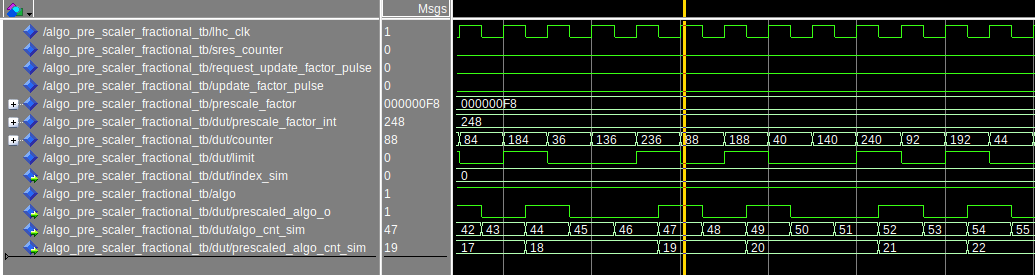
\includegraphics[width=15cm]{figures/Screenshot_fractional_prescalers}
\caption{Fractional prescaler}
\label{fig:fdl:fractional_prescalers}
\end{figure}

In Figure (\ref{fig:fdl:fractional_prescalers}) one can see the simulation of a fractional prescaler. In this example the fractional prescale factor is 2.48 and the signal
”prescale factor int” shows this value multiplied by 10\textsuperscript{\tiny{precision}}, i.e., currently by 100 (so, 248).
The signal ”algo” is always true, in other words, without prescale this Algorithm would be firing (sending a trigger request) in every bunch crossing. Signal ”prescaled algo o” shows when the trigger request of the prescaled Algorithm is allowed to pass. Signals ”algo cnt sim” and ”prescaled algo cnt sim” show the number of this Algorithm’s trigger requests before and after the prescale logic. At the cursor point a factor 47/19 (\~{=} 2.4737) is reached. With ”algo cnt sim” reaching higher numbers, on average the effective prescale factor gets closer and closer to the requested value of 2.48.

\subsubsection{Finor-masks}
\label{sec:fdl:finor_masks}

Every Algorithm passes a \finor-mask, which enables the Algorithm for \finor.
The \finor-masks are implemented as registers (\ref{masks_regs}) and loaded at the begin of a run.\\
Configuration of \finor-masks is done by a "run settings key" (e.g. UGT\_RS\_KEYS => ugt\_rs\_algo\_finor\_mask\_empty/v4)

\subsubsection{Veto-masks}
\label{sec:fdl:veto_masks}

Every Algorithm passes a veto-mask, if at least one Algorithm, which is enabled by veto-mask, becomes high state, then \finor is disabled as long as the Algorithm is in high state.
The veto-masks are implemented as registers (\ref{masks_regs}) and loaded at the begin of a run.\\
Configuration of veto-masks is done by a "run settings key" (e.g. UGT\_RS\_KEYS => ugt\_rs\_algo\_finor\_veto\_all\_zero/v2)

\subsubsection{Finor}
\label{sec:fdl:finor}

The \finor-signal is a disjunction of all Algorithms passed the \finor-bx-masks. An Algorithm enabled by veto-mask, disables the \finor. This is done on the FINOR-AMC502 module.

\clearpage
\subsubsection{Registers and memories}
\label{sec:fdl:reg_mem}

All registers and memories are 32 bits wide. (Definition of addresses is shown in Table~\ref{tab:fdl:ufdl_register_map}.)

\begin {itemize}
\item Dual-port memories for the algo-bx-masks are implemented. For each Algorithm there is a mask bit at every bunch crossing of one orbit. Therefore in total memories of 4096 x 512 bits
are implemented. Because of the 32 bit data interface, 16 memories each with a size of 4096 x 32 bits are instantiated.
\item Read-only registers for the value of rate-counters (before and after prescalers, post-dead-time counters) are implemented, 512 registers, one for every Algorithm. Rate-counter value has 32 bits.
\item Registers for prescale factor of the prescalers are implemented, 512 registers, one for every Algorithm. A prescale factor value has 24 bits.
\item Registers for masks (\finor- and veto-masks) are implemented, 512 registers.
\item One register for prescale factors set index is implemented. This register contains a value, which is unique for a given set of prescale factors. The content of this register is
part of \record.
\item One register for command pulses is implemented. One bit of this register (bit 0) is used for "setting the request signal for updating prescale factors high", which enables, that the prescale factors and the prescale factor set index
are loaded at the begin of a luminosity segment period. (Other bits are not defined yet.)
\item One control register is implemented (the content has to be defined).
\item 32 register for L1 Trigger Menu name for \ugtl is implemented.
\item 4 register for L1 Trigger Menu UUID for \ugtl is implemented.
\item One register for L1 Trigger Menu compiler version is implemented.
\item One register for \ufdl firmware version is implemented.
\item One register for \ugtl firmware (fixed code) version is implemented.
\end {itemize}

\paragraph{Register map}
\label{sec:fdl:reg_map}
The register map for \ufdl has a base address of \verb|0x90000000|.

\textbf{Remark:}\\
Register "SVN revision number" is used for firmware version of Framework VHDL code (SVN revision number is obsolete).

% % HB 2016-11-03: inserted "longtable"
\begin{longtable}{c p{.27\columnwidth} c p{.43\columnwidth}}
\caption{\ufdl register map}\\
\hline
Offset & {Register name} & {Access} & {Description}\\
\hline
\hline
\endhead
0x90000000 & \verb|Algo BX masks(0)| & r/w & 4096 memory addresses of algo-bx-masks for Algorithms 0-31.\\
0x90001000 & \verb|Algo BX masks(1)| & r/w & 4096 memory addresses of algo-bx-masks for Algorithms 32-63.\\
... & ... & ... & ...\\
0x9000F000 & \verb|Algo BX masks(15)| & r/w & 4096 memory addresses of algo-bx-masks for Algorithms 480-511.\\
0x90010000 & \vtop{\hbox{\strut \verb|Rate counter|}\hbox{\strut \verb|before prescaler|}} (\ref{rate_counter_before_prescaler_regs}) & r & 512 read-only registers for rate-counter values before prescalers.\\
0x90010200 & \verb|Prescale factors| (\ref{prescale_factor_regs}) & r/w & 512 registers for prescale factors.\\
0x90010400 & \vtop{\hbox{\strut \verb|Rate counter|}\hbox{\strut \verb|after prescaler|}} (\ref{rate_counter_after_prescaler_regs}) & r & 512 read-only registers for rate-counter values after prescalers.\\
0x90010600 & \vtop{\hbox{\strut \verb|Rate counter|}\hbox{\strut \verb|post-dead-time|}} (\ref{rate_counter_pdt_regs}) & r & 512 read-only registers for post-dead-time rate-counter values.\\
0x90010800 & \verb|Masks| (\ref{masks_regs}) & r/w & 512 registers for \finor-masks and veto-masks. Bit 0 = \finor-mask, bit 1 = veto-mask.\\
0x90091880 & \vtop{\hbox{\strut \verb|Prescale factors|}\hbox{\strut \verb|set index|}} (\ref{prescale_factor_set_index_reg}) & r/w & Register for prescale factors set index.\\
% 0x90091888 & \verb|Control| & r/w & Register for control signals (content has to be defined !!!).\\
0x900918C0 & \verb|L1tm name| & r & 32 registers for L1 Trigger Menu name for \ugtl.\\
0x900918E0 & \verb|L1tm uuid| & r & 4 registers for L1 Trigger Menu UUID for \ugtl.\\
0x900918E4 & \vtop{\hbox{\strut \verb|L1tm compiler|}\hbox{\strut \verb|version|}} (\ref{L1tm_compiler_version_reg}) & r & Register for L1 Trigger Menu compiler version.\\
0x900918E5 & \verb|GTL FW version| (\ref{gtl_fw_version_reg}) & r & Register for firmware version of \ugtl VHDL code.\\
0x900918E6 & \verb|FDL FW version| (\ref{fdl_fw_version_reg}) & r & Register for firmware version of \ufdl VHDL code.\\
0x900918E7 & \verb|L1tm FW uuid| & r & 4 registers for L1 Trigger Menu FW UUID for \ugtl.\\
0x900918EB & \verb|SVN revision number| & r & Register for firmware version of framework VHDL code.\\
0x900918EC & \verb|L1tm uuid hash| & r & Register for L1 Trigger Menu UUID hash for \ugtl.\\
0x900918ED & \verb|L1tm FW uuid hash| & r & Register for L1 Trigger Menu FW UUID hash for \ugtl.\\
0x900918EE & \verb|Module ID| & r & Register for Module ID of L1 Trigger Menu.\\
0x90091900 & \verb|Command Pulses| (\ref{command_pulses_reg}) & r/w & \vtop{\hbox{\strut Register for command pulses}\hbox{\strut (request\_update\_factor\_pulse).}}\\
0x90091980 & \verb|Rate counter finor| (\ref{rate_counter_finor_regs}) & r & One read-only registers for finor rate-counter value.\\
0x90092200 & \verb|L1A latency delay| (\ref{l1a_latency_delay_reg}) & r/w & Register for L1A latency delay value (used for post-dead-time counter).\\
0x90093000 & \verb|Rate counter L1A| (\ref{rate_counter_l1a_reg}) & r & One read-only registers for L1A rate-counter value.\\
0x90094000 & \verb|Rate counter veto| (\ref{rate_counter_veto_reg}) & r & One read-only registers for veto rate-counter value.\\
0x90095000 & \vtop{\hbox{\strut \verb|Current prescale|}\hbox{\strut \verb|set index|}} (\ref{current_prescale_factor_set_index_updated_reg}) & r & Read-only register for prescale factors set index, which was "updated" with begin of current lumi-section ("prescale\_factors\_set\_index\_reg\_updated(0)" in VHDL).\\
0x90095001 & \vtop{\hbox{\strut \verb|Previous prescale|}\hbox{\strut \verb|set index|}} (\ref{previous_prescale_factor_set_index_updated_reg}) & r & Read-only register for prescale factors set index, which was "updated" with begin of previous lumi-section for monitoring "prescale\_factors\_set\_index\_reg\_updated(1)" in VHDL).\\
0x90096000 & \vtop{\hbox{\strut \verb|Calibration trigger|}\hbox{\strut \verb|gap|}} (\ref{calibration_trigger_gap_reg}) & r/w & Register for begin and end (in Bx) of calibration trigger gap.\\
\hline
\label{tab:fdl:ufdl_register_map}
\end{longtable}

\begin{register}{htbp}{Rate counter before prescaler}{}
	\label{rate_counter_before_prescaler_regs}%
	\regfield{rate\_counter\_before\_prescaler}{32}{0}{0}%
	\reglabel{Reset}\regnewline%

	\begin{regdesc}
% 	\begin{reglist}[Request~Depth]
	\begin{reglist}
		\item [rate\_counter\_before\_prescaler] Rate counter before prescaler. Counts the occurancy of an algo (given by register address) in one luminosity segment.
	\end{reglist}
	\end{regdesc}
\end{register}

\begin{register}{htbp}{Prescale factor}{}
	\label{prescale_factor_regs}%
	\regfield{reserved}{8}{24}{0}%
	\regfield{prescale\_factor}{24}{0}{1}%
	\reglabel{Reset}\regnewline%

	\begin{regdesc}
% 	\begin{reglist}[Request~Depth]
	\begin{reglist}
		\item [prescale\_factor] Prescale factor of an algo (given by register address). Prescale factor = 0 means "disable alg". The factor has a precision of two digits after comma, therefore values in register are equal to factor * 100 (e.g.: factor=1.00 => 100 [0x64]).
	\end{reglist}
	\end{regdesc}
\end{register}

\begin{register}{htbp}{Rate counter after prescaler}{}
	\label{rate_counter_after_prescaler_regs}%
	\regfield{rate\_counter\_after\_prescaler}{32}{0}{0}%
	\reglabel{Reset}\regnewline%

	\begin{regdesc}
% 	\begin{reglist}[Request~Depth]
	\begin{reglist}
		\item [rate\_counter\_after\_prescaler] Rate counter after prescaler. Counts the occurancy of an algo (given by register address) in one luminosity segment.
	\end{reglist}
	\end{regdesc}
\end{register}

\begin{register}{htbp}{Rate counter post-dead-time}{}
	\label{rate_counter_pdt_regs}%
	\regfield{rate\_counter\_postdeadtime}{32}{0}{0}%
	\reglabel{Reset}\regnewline%

	\begin{regdesc}
% 	\begin{reglist}[Request~Depth]
	\begin{reglist}
		\item [rate\_counter\_postdeadtime] Rate counter post-dead-time. Counts the occurancy of an algo (given by register address) and L1A at the same bx in one luminosity segment.
	\end{reglist}
	\end{regdesc}
\end{register}

\begin{register}{htbp}{Masks}{}
	\label{masks_regs}%
	\regfield{reserved}{30}{2}{0}%
	\regfield{veto\_mask}{1}{1}{0}%
	\regfield{finor\_mask}{1}{0}{1}%
	\reglabel{Reset}\regnewline%

	\begin{regdesc}
% 	\begin{reglist}[Request~Depth]
	\begin{reglist}
		\item [veto\_mask] Selection of a veto (by an algo, given by register address) for veto-or.
		\item [finor\_mask] Selection of an algo (given by register address) for final-or.
	\end{reglist}
	\end{regdesc}
\end{register}

\begin{register}{htbp}{Prescale factors set index}{}
	\label{prescale_factor_set_index_reg}%
	\regfield{reserved}{24}{8}{0}%
	\regfield{prescale\_factor\_set\_index}{8}{0}{0}%
	\reglabel{Reset}\regnewline%

	\begin{regdesc}
	\begin{reglist}
		\item [prescale\_factor\_set\_index] Index for a certain set of prescale factors.
	\end{reglist}
	\end{regdesc}
\end{register}

\begin{register}{htbp}{L1tm compiler version}{}
	\label{L1tm_compiler_version_reg}%
	\regfield{reserved}{8}{24}{0}%
	\regfield{major}{8}{16}{0}%
	\regfield{minor}{8}{8}{0}%
	\regfield{revision}{8}{0}{0}%
	\reglabel{Reset}\regnewline%

	\begin{regdesc}
	\begin{reglist}
		\item [major] Major version of VHDL producer.
		\item [minor] Minor version of VHDL producer.
		\item [revision] Revision version of VHDL producer.
	\end{reglist}
	\end{regdesc}
\end{register}

\begin{register}{htbp}{GTL FW version}{}
	\label{gtl_fw_version_reg}%
	\regfield{reserved}{8}{24}{0}%
	\regfield{major}{8}{16}{0}%
	\regfield{minor}{8}{8}{0}%
	\regfield{revision}{8}{0}{0}%
	\reglabel{Reset}\regnewline%

	\begin{regdesc}
% 	\begin{reglist}[Request~Depth]
	\begin{reglist}
		\item [major] Major version of GTL firmware.
		\item [minor] Minor version of GTL firmware.
		\item [revision] Revision version of GTL firmware.
	\end{reglist}
	\end{regdesc}
\end{register}

\begin{register}{htbp}{FDL FW version}{}
	\label{fdl_fw_version_reg}%
	\regfield{reserved}{8}{24}{0}%
	\regfield{major}{8}{16}{0}%
	\regfield{minor}{8}{8}{0}%
	\regfield{revision}{8}{0}{0}%
	\reglabel{Reset}\regnewline%

	\begin{regdesc}
% 	\begin{reglist}[Request~Depth]
	\begin{reglist}
		\item [major] Major version of FDL firmware.
		\item [minor] Minor version of FDL firmware.
		\item [revision] Revision version of FDL firmware.
	\end{reglist}
	\end{regdesc}
\end{register}

\begin{register}{htbp}{Command Pulses Register}{}
	\label{command_pulses_reg}%
	\regfield{reserved}{31}{1}{0}%
	\regfield{request\_update\_factor\_pulse}{1}{0}{0}%
	\reglabel{Reset}\regnewline%

	\begin{regdesc}
% 	\begin{reglist}[Request~Depth]
	\begin{reglist}
		\item [request\_update\_factor\_pulse] A sequence of applying 1 followed by 0 generates the "request update factors pulse". (Updating is done at the next "begin of luminosity segment".)
	\end{reglist}
	\end{regdesc}
\end{register}

\begin{register}{htbp}{Rate counter finor}{}
	\label{rate_counter_finor_regs}%
	\regfield{rate\_counter\_finor}{32}{0}{0}%
	\reglabel{Reset}\regnewline%

	\begin{regdesc}
% 	\begin{reglist}[Request~Depth]
	\begin{reglist}
		\item [rate\_counter\_finor] Rate counter finor. Counts the occurancy of finor in one luminosity segment.
	\end{reglist}
	\end{regdesc}
\end{register}

\begin{register}{htbp}{L1A latency delay}{}
	\label{l1a_latency_delay_reg}%
	\regfield{reserved}{24}{6}{0}%
	\regfield{l1a\_latency\_delay}{6}{0}{0}%
	\reglabel{Reset}\regnewline%

	\begin{regdesc}
% 	\begin{reglist}[Request~Depth]
	\begin{reglist}
		\item [l1a\_latency\_delay] L1A latency delay value (used for post-dead-time counter).
	\end{reglist}
	\end{regdesc}
\end{register}

\begin{register}{htbp}{Rate counter L1A}{}
	\label{rate_counter_l1a_reg}%
	\regfield{rate\_counter\_l1a}{32}{0}{0}%
	\reglabel{Reset}\regnewline%

	\begin{regdesc}
% 	\begin{reglist}[Request~Depth]
	\begin{reglist}
		\item [rate\_counter\_l1a] Rate counter L1A. Counts the occurancy of L1A in one luminosity segment.
	\end{reglist}
	\end{regdesc}
\end{register}

\begin{register}{htbp}{Rate counter veto}{}
	\label{rate_counter_veto_reg}%
	\regfield{rate\_counter\_veto}{32}{0}{0}%
	\reglabel{Reset}\regnewline%

	\begin{regdesc}
% 	\begin{reglist}[Request~Depth]
	\begin{reglist}
		\item [rate\_counter\_veto] Rate counter veto. Counts the occurancy of veto in one luminosity segment.
	\end{reglist}
	\end{regdesc}
\end{register}

\begin{register}{htbp}{Current prescale set index}{}
	\label{current_prescale_factor_set_index_updated_reg}%
	\regfield{reserved}{24}{8}{0}%
	\regfield{prescale\_factor\_set\_index\_updated}{8}{0}{0}%
	\reglabel{Reset}\regnewline%

	\begin{regdesc}
% 	\begin{reglist}[Request~Depth]
	\begin{reglist}
		\item [prescale\_factor\_set\_index\_updated] Index for a certain set of prescale factors, which was "updated" with begin of current lumi-section.
	\end{reglist}
	\end{regdesc}
\end{register}

\begin{register}{htbp}{Previous prescale set index}{}
	\label{previous_prescale_factor_set_index_updated_reg}%
	\regfield{reserved}{24}{8}{0}%
	\regfield{prescale\_factor\_set\_index\_updated}{8}{0}{0}%
	\reglabel{Reset}\regnewline%

	\begin{regdesc}
% 	\begin{reglist}[Request~Depth]
	\begin{reglist}
		\item [prescale\_factor\_set\_index\_updated] Index for a certain set of prescale factors, which was "updated" with begin of previous lumi-section.
	\end{reglist}
	\end{regdesc}
\end{register}

\begin{register}{htbp}{Calibration trigger gap}{}
	\label{calibration_trigger_gap_reg}%
	\regfield{reserved}{4}{28}{0}%
	\regfield{end\_calibration\_trigger\_gap}{12}{16}{0}%
	\regfield{reserved}{4}{12}{0}%
	\regfield{begin\_calibration\_trigger\_gap}{12}{0}{0}%
	\reglabel{Reset}\regnewline%

	\begin{regdesc}
	\begin{reglist}
		\item [begin\_calibration\_trigger\_gap] Begin of calibration trigger gap (in Bx).
		\item [end\_calibration\_trigger\_gap] End of calibration trigger gap (in Bx).
	\end{reglist}
	\end{regdesc}
\end{register}

\clearpage

